\section{Experiments}
\label{sec:results}

\paragraph{Design.}
In every arm the teleoperated half carries the robot's encoder labels; only the glove half carries the camera under test, and its observation is whichever camera the arm deploys. Table~\ref{tab:arms} lists the eight arms. Arms 1--4 are the device and its budget pair; arm 6 checks the labels; arms 5, 7 and 8 compare cameras, arm 5 being the conventional wrist-camera recipe \citep{chi2024umi}. All glove arms train on the same 198 demonstrations. Arms 5 and 8 observe through a wrist fisheye that was mounted on the glove for this ablation only; the head-view arms use the glove with no electronics. The fixed-camera arms train on \SI{10}{\percent} fewer glove frames (43.5k against 48.5k), which is the occlusion cost of the fixed camera and not a budget choice.

\begin{table}[t]
  \centering
  \footnotesize
  \caption{The eight policies. Teleop labels are encoders except arm 6. Robot val = ACT loss on the 6 held-out teleoperated episodes (encoder targets, comparable across all rows; arm 6 is scored on the encoder targets too). Rollouts: \grid{25} placements, one trial each, \SI{60}{s} budget; failure modes n = no grasp, d = dropped before the bin, b = dropped at the bin. \todo{fill from the grid}}
  \label{tab:arms}
  \setlength{\tabcolsep}{4pt}
  \begin{tabular}{clllcccl}
    \toprule
    \# & arm & glove labels & observation & teleop + glove & val & success & fails \\
    \midrule
    1 & teleop only & --- & head cam & 172 & 0.318 & \grid{/25} & \grid{} \\
    2 & \textbf{device} & head cam & head cam & 172 + 194 & \textbf{0.263} & \grid{/25} & \grid{} \\
    3 & teleop only, low budget & --- & head cam & 48 & 0.464 & \grid{/25} & \grid{} \\
    4 & device, low budget & head cam & head cam & 48 + 194 & 0.295 & \grid{/25} & \grid{} \\
    5 & wrist-camera UMI & fixed cam & wrist fisheye & 168 + 253 & 0.257 & \grid{/25} & \grid{} \\
    6 & head-cam teleop labels & --- & head cam & 172 (head labels) & 0.328 & \grid{/25} & \grid{} \\
    7 & fixed camera as system & fixed cam & fixed cam & 172 + 255 & 0.256 & \grid{/25} & \grid{} \\
    8 & head labels, wrist view & head cam & wrist fisheye & 168 + 192 & 0.252 & \grid{/25} & \grid{} \\
    \bottomrule
  \end{tabular}
\end{table}

\paragraph{Label accuracy.}
With the ball on the YAM and the encoders as reference, the head-camera chain places the tool point with \SI{6.5}{mm} median / \SI{14.1}{mm} p90 error and \SI{1.55}{\degree} / \SI{2.70}{\degree} rotation (5\,065 frames, \SI{91}{\percent} inliers), after the one-time base link absorbs the constant offset. The jaw width is checked the same way: on 112 teleoperated episodes (24.6k frames) the head-camera width is within \SI{3.5}{\percent} of the stroke of the encoder value at the median (\SI{7.9}{\percent} p90; about 3 and \SI{7.5}{mm} of the \SI{95}{mm} stroke), \SI{2.3}{\percent} in the closed state that decides a grasp, with no lag (a one-frame shift raises the error) and a label on every frame in 9 of 10 episodes (worst \SI{68}{\percent}). The residual is a systematic under-read of \SI{4}{}--\SI{6}{\percent} at full opening, a scale error of the per-session fit rather than noise. \todo{Yuan: a check on unseen openings across viewing angles, with coverage per angle, would make this a proper instrument table.} Downstream, a policy trained on head-camera labels instead of encoders (arm 6 against arm 1), scored on the same encoder-labelled held-out episodes, reaches 0.328 against 0.318, a \SI{3}{\percent} price for the labels, and succeeds in \grid{X/25} rollouts against \grid{X/25}.

\paragraph{Co-training and the teleoperation budget.}
Glove and teleoperated episodes are co-trained as one merged dataset, as robot data from different sources has been before \citep{fu2024mobilealoha,kareer2025egomimic}. Adding the glove set to all 172 teleoperated episodes lowers the robot-validation loss from 0.318 to 0.263 (\SI{17}{\percent}); added to 48 teleoperated episodes it lowers it from 0.464 to 0.295. Fig.~\ref{fig:budget} shows the full curve: the glove set is worth 65--100 teleoperated episodes by log-linear interpolation of the teleop-only curve, i.e. 2--3 glove demonstrations per teleoperated one, and the 48-episode mix lands between 96 and 172 teleoperated episodes alone. In robot time, the glove set saves about 50--120 teleoperated episodes at the 48-episode budget.The gain shrinks with budget (0.075 at 24 episodes down to 0.011 at 96, measured against the full mix), so glove data stretches a small teleoperated set but does not replace the last few dozen episodes. On the robot \grid{the 48-episode mix succeeds in X/25 against X/25 for the 48 teleoperated episodes alone and X/25 for the full 172}, \todo{with the recovery behaviour of the mix: in scene 5 the mix missed its first grasp, backed off and re-grasped, where the teleop-only policy never closed in}.

\begin{figure}[t]
  \centering
  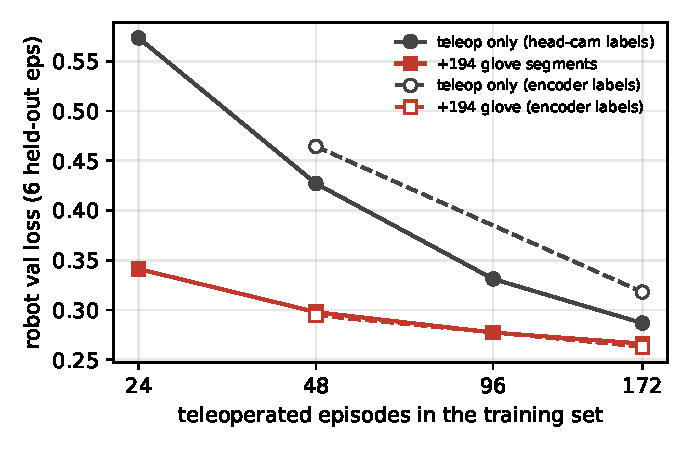
\includegraphics[width=0.6\linewidth]{fig/budget.pdf}
  \caption{Robot validation loss against the number of teleoperated episodes, with and without the 194 glove segments. Solid: head-camera-labelled teleoperation (round-2 chain, four budgets); dashed: encoder-labelled teleoperation (final design, two budgets). The glove set moves every budget to the level of 2--4$\times$ as many teleoperated episodes.}
  \label{fig:budget}
\end{figure}

\paragraph{Which camera.}
Offline, the four co-trained arms with different cameras (2, 5, 7, 8) sit within 0.011 of each other, and each gains 0.04--0.06 over its teleop-only twin, so the validation loss does not separate the cameras; offline loss is known to be a weak proxy for rollout success \citep{mandlekar2021robomimic}. The rollouts do. \grid{Arm 2 succeeds in X/25, the wrist-camera recipe in X/25, the fixed camera in X/25, and head labels on the wrist view in X/25.} The failure modes split by camera: head-view policies fail by never grasping, wrist-view policies by dropping the block during the carry, \grid{d+b = X of Y failures for arms 5 and 8 against X of Y for arms 1--4}. \todo{every observed wrist-view drop happened while the bin was outside the fisheye's view; no drop was observed with the bin in view; the head camera keeps gripper and bin in frame throughout the carry.} Holding the labels fixed (arm 8 against arm 2) isolates the observation; holding the observation fixed (arm 8 against arm 5) isolates the label source: \grid{result}. The fixed camera (arm 7) \grid{result}; note that it was mounted low because the positioner occupied the elevated vantage point, so its occlusion rate is an upper bound for a fixed camera in this workspace.

\begin{figure}[t]
  \centering
  \fbox{\parbox[c][4.2cm][c]{0.96\linewidth}{\centering \todo{Rollout protocol figure as in the device paper: the 25 placements with per-scene success over the 8 arms; ghost-alignment inset. Generate from rollout\_logs/grid\_20261016 (placements.json, scene*\_ref.png, trials.jsonl).}}}
  \caption{Rollout protocol. \grid{25} placements, each scene's block re-placed to a saved reference for every arm (ghost alignment), arm order shuffled per scene, \SI{60}{s} budget.}
  \label{fig:placements}
\end{figure}

\paragraph{Anecdotes.}
\todo{Transcribe from rollout\_logs/grid\_20261016/anecdotes.md: scene-5 budget pair; mix\_gHA opening mid-carry with the block out of view; wrist drops only when the bin is out of view.}
